\documentclass[9pt, table]{beamer}
  \usetheme[block=fill]{metropolis}  % https://github.com/matze/mtheme

\usepackage{amsmath}
\usepackage{amssymb}
\usepackage{mathtools}
\usepackage{xcolor}
\usepackage{csquotes}
\usepackage{url}

\title{Machine Learning}
\date{}
\author{Thorben Menne}

\newcommand{\deriv}[1]{\mathrm{d}#1}
\newcommand{\dderiv}[2]{\frac{\mathrm{d}#1}{\mathrm{d}#2}}
\newcommand{\del}[1]{\partial #1}
\newcommand{\ddel}[2]{\frac{\partial #1}{\partial #2}}

\newcommand{\tcw}[1]{\textcolor{white}{#1}}
\newcommand{\tcb}[1]{\textcolor{black}{#1}}
\newcommand{\ccw}{\cellcolor{white}}
\newcommand{\ccga}{\cellcolor{black!50}}
\newcommand{\ccgb}{\cellcolor{black!40}}
\newcommand{\ccgc}{\cellcolor{black!30}}
\newcommand{\ccb}{\cellcolor{black}}

% Buffer slides for subsections (tex.stackexchange.com/questions/117658)
\AtBeginSubsection[]{
  \begin{frame}
    \subsectionpage
  \end{frame}
}


% Main title, author etc. in header
\subtitle{Part II -- Machine Learning Basics\\\vspace*{1.5ex}
  \small \textbf{Goal:} Gain basic understanding on why we need machine learning, what the differences between the many algorithms is and get introduced to some popular approaches
}

\begin{document}
  % Input after \begin{document} needs mdframed, listings, xcolor package
  % Make code snippets dark with rounded mdframe
  \mdfsetup{%
    backgroundcolor=col_bg,
    roundcorner=5pt,
    innerleftmargin=2em,  % 1em is for numbers
    innerrightmargin=1em,
    innertopmargin=0ex,
    innerbottommargin=0ex,
    skipabove=0.5\baselineskip,
    skipbelow=0.5\baselineskip,
  }
  \lstset{
    language=Python,  % Standard language
    inputpath=snippets,  % Where to search for lstinputlisting files
    tabsize=4,
    showspaces=false,  % Show space hints
    showstringspaces=true,
    numbers=left,  % Line numbering
    numbersep=1em,
  }
  \lstdefinestyle{dark}{%
    title=\lsttitledark{\lstname},
    basicstyle=\color{col_fg}\footnotesize\ttfamily,
    numberstyle=\color{col_fg}\tiny,
    commentstyle=\color{col_comment},
    % identifierstyle=\color{col_identifier},  % Not defined for Python
    keywordstyle=\color{col_keyword}\bfseries,
    stringstyle=\color{col_string},
    backgroundcolor=\color{col_bg},
    emph={range, enumerate},  % Additional coloring for given keywords
    emphstyle=\color{col_emph},
  }
  \lstdefinestyle{plain}{%
    numbers=none,
    basicstyle=\footnotesize\ttfamily,
    numberstyle=\tiny,
  }
  \maketitle

% %%%%%%%%%%%%%%%%%%%%%%%%%%%%%%%%%%%%%%%%%%%%%%%%%%%%%%%%%%%%%%%%%%%%%%%%%%%%%
% Intro
% %%%%%%%%%%%%%%%%%%%%%%%%%%%%%%%%%%%%%%%%%%%%%%%%%%%%%%%%%%%%%%%%%%%%%%%%%%%%%
\section{Introduction}

  \begin{frame}{Fitting a line to data}
    \begin{columns}
      \begin{column}{0.5\textwidth}
        \begin{itemize}
          \item One of the most basic but also often needed questions: I have some data points, which line fits them best?
          \item This is a classical supervised regression learning algorithm (although it's usually not called this way)
          \item Can be solved using maximum likelihood parameter estimation
          \begin{itemize}
            \item In case you think more of least squares: LSQ can be obtained as a special case of likelihood fitting using a Gaussian model for the data points
          \end{itemize}
          \item An analytic solution exist for this exact problem by maximizing
          \begin{equation*}
            \argmax_{\theta}\mathcal{L} \propto \prod_i
              \frac{1}{\sqrt{2\pi}\sigma}
              \exp{-\frac{(y_i - f(x_i|\theta))^2}{2\sigma^2}}
          \end{equation*}
          where the parameters only appear linear in $f$
        \end{itemize}
      \end{column}

      \begin{column}{0.5\textwidth}
        \includegraphics[width=\textwidth]{02-img-fit_straight_line_example}
      \end{column}

    \end{columns}
  \end{frame}

  \begin{frame}{Maximum Likelihood estimation}
    \begin{itemize}
      \item In general the idea of maximum Likelihood estimation (MLE) is to tune the model parameters so that the data appears to be most likely to originate from the tuned model
      \item This is expressed by maximizing the expression
        \begin{equation*}
          \mathcal{L}(x|\theta) = \prod_{i=1}^N f(x_i | \theta)
        \end{equation*}
        which is just the product of the PDF value for each of the $i=1, \dots, N$ data points $x_i$.
      \item For numerical reasons, almost always the negative log-Likelihood is minimized instead
      \begin{equation}
        -\ln\mathcal{L}(x\theta) = -\sum_{i=1}^N \ln(f(x_i | \theta))
      \end{equation}
      \item Some simple LLH parameter estimates can be derived analytically, like the straight line fit before, most are too complicated and require numerical solutions
      \item Note: The model selection is crucial in MLE, it incorporates all the knowledge we have of the estimated process, for example physical conditions
      \item Depending on the model, MLE can be used for regression as well as classification tasks
    \end{itemize}
  \end{frame}

  \begin{frame}{Maximum Likelihood example plot}
    \includegraphics[width=\textwidth]{02-img-likelihood_estimation_example}
  \end{frame}

  \begin{frame}{Logistic Regression}
    \begin{columns}
      \begin{column}{0.65\textwidth}
        \begin{itemize}
          \item In regression problems, like the line fit seen previously, it is tried to minimize the distance between the model and the data points
          \item However, in classification problems, data usually comes in discrete categories, also called classes
          \item These (binary) classes can be encoded with $Y\in {0, 1}$ (eg. sun will shine: $y=1$, sun won't shine: $y=0$), also called \enquote{one-hot-encoding}
          \item We can't simply fit a line to those data point, because the model would be meaningless
          \item \textbf{The way around: Logistic Regression}, which is, actually, a classification algorithm but uses regression to arrive there
          \item We use our Likelihood framework again, but we need to adapt our model to take the discrete classes into account
          % \item \emph{Note:} Regression and classification task are more or less the same, only with a difference in the choice of model.
          % Both operate within the Likelihood framework
        \end{itemize}
      \end{column}
      \begin{column}{0.35\textwidth}
        \includegraphics[width=\textwidth]{02-img-logit}
      \end{column}
    \end{columns}
  \end{frame}

  \begin{frame}{Logistic Regression}
    \begin{columns}
      \begin{column}{0.65\textwidth}
        \begin{itemize}
          \item Using a modified Bernoulli LLH with a model of the success probability $p$ for a given $x_i$ rather than individual $p_i$ gives
          \begin{equation*}
            \mathcal{L} = \prod_i
              p(x_i | \theta)^{y_i} (1 − p(x_i | \theta))^{1 − y_i}
          \end{equation*}
          \item The most simple assumption for the model $p(x_i | \theta)$ is making it linear again, but now with a slight twist
          \begin{itemize}
            \item Because we want our model to predict between one and zero, not $p$ is assumed to be linear, but the expression $\ln{p / (1 - p)}$ (the \emph{logit} function)
            \item This seems arbitrary but, $p / (1 - p)$ are the odds and using the logarithm is a \enquote{natural} choice for extending the range to $[-\infty, \infty]$
          \end{itemize}
          \item We can then set
            \begin{equation}
              \ln \frac{p}{1 - p} = \theta x \Leftrightarrow
                p(x | \theta) = \frac{1}{1 + \exp(-\theta x)}
            \end{equation}
            which can be plugged into the Likelihood defined above
        \end{itemize}
      \end{column}
      \begin{column}{0.35\textwidth}
        \includegraphics[width=\textwidth]{02-img-logit}
      \end{column}
    \end{columns}
  \end{frame}

  \begin{frame}{Logistic Regression example plot}
    \includegraphics[width=\textwidth]{02-img-logistic_regression}
  \end{frame}

  \begin{frame}{Why do we need ML then?}
    \begin{columns}[c]
      \begin{column}{0.8\textwidth}
        \begin{itemize}
          \item With the maximum Likelihood formalism we have a very versatile and mighty tool at our hands
          \begin{itemize}
            \item It can be used to model regression and even classification tasks and estimate optimal parameters
            \item There is also a whole class of algorithms utilizing Bayes theorem to make posterior predictions (not covered here)
          \end{itemize}
          \item \textbf{So why do we need machine learning at all then?}
          \item For complex tasks, model building becomes equivalently complex
          \begin{itemize}
            \item How to write down a model for recognizing items in images?
              Potentially impossible to craft manually
            \item Model must be robust against rotation, translation, scaling, color variations, lightning variations, variations in the item itself, etc, etc ...
          \end{itemize}
          \item Big advantage of machine learning, aka the \enquote{learning}: Using an algorithm that \enquote{learns} the model itself by some kind of predefined measure (aka loss function) from a given dataset representing examples from the target distribution
          \begin{itemize}
            % \item Note: The term \enquote{learning} should not be understood to mean the same as human learning generally means.
            \item In general, the models are so general, that they adapt to many problems with very good performance
            \item In the end, it's \emph{just curve fitting}
          \end{itemize}
        \end{itemize}
      \end{column}
      \begin{column}{0.2\textwidth}
        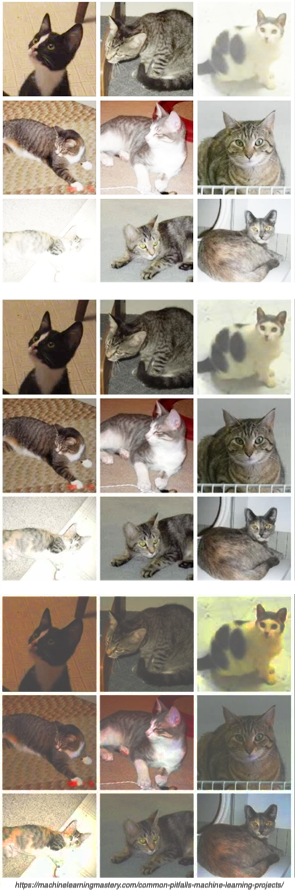
\includegraphics[height=0.9\textheight]{02-img_cat_examples}
      \end{column}
    \end{columns}
  \end{frame}

  \begin{frame}{Different tasks to solve with ML}
    Different task in which machine learning algorithms are used (not complete):
    \begin{description}
      \item [Classic classification] Sorting inputs in previously specified $k$ classes.
        Typically resembles a function $\mathbb{R}^n \rightarrow \{1, \dots, k\}$
      \item [Classic regression] The other classical task, predicting a continuous value from the input, typically $\mathbb{R}^n \rightarrow \mathbb{R}$
      \item [Transcription] Converting some kind of rather unstructured input (voice, text in image, etc.) in textual form (heavily used in modern speech recognition)
      \item [Translation] Translating between languages.
        Set in the field of natural language processing.
      \item [Anomaly detection] Noticing any kind of unusual behaviour or outliers in input data
      \item [Synthesis] Generating new data that looks similar to previously shown data.
        Eg. \emph{Deep Fake} or speech synthesis.
      \item [Filling of missing values] Filling \enquote{holes} in input data.
        Can be used to patch images with missing data or similar tasks
      \item [Denoising] Reducing noise in input data, for example in super resolution or also speech recognition
    \end{description}
  \end{frame}

  \begin{frame}{Supervised / unsupervised learners}
    \begin{columns}[t]
      \begin{column}{0.65\textwidth}
        \begin{itemize}
          % \item Machine learning algorithms can roughly be separated into \emph{supervised} and \emph{unsupervised} algorithms
          \item \textbf{Supervised algorithms} are given a training data set with known labels
          \begin{itemize}
            \item In each learning step, the algorithm can compare its results to the ground truth, adapt and get better over time
            \item Popular example algorithms are: Naive Bayes, k-nearest neighbour, support vector machines, tree based learners, Neural Networks, linear discriminants and again linear regression
          \end{itemize}
          \item \textbf{Unsupervised algorithms} aim to work on datasets with no class information available  % and try to reduce the need for human oversight to a minimum
          \begin{itemize}
            \item Not being able to learn from a ground truth, such models usually try to find a representation of the underlying data distribution.
            \item Clustering algorithms, like k-means, try to group data points based on some distance measure
              % Cross validation can be used to estimate hyper-parameters like the number of clusters to find
            \item Neural network autoencoders try to find a compressed version of the input by piping the data through a bottleneck and then reconstructing them from that reduced input.
              % They can thus compare the input to their own generated output
            \item \emph{Expectation-maximization} is an iterative Likelihood method and eg. used in Gaussian mixture models
          \end{itemize}
          % \item Here focus mostly on an overview of supervised learners
        \end{itemize}
      \end{column}
      \begin{column}{0.35\textwidth}
        \vspace*{1em}
        \includegraphics[width=\textwidth]{02-img-supervised_unsupervised_comic}
      \end{column}
    \end{columns}
  \end{frame}

  \begin{frame}{Info graphic supervised}
      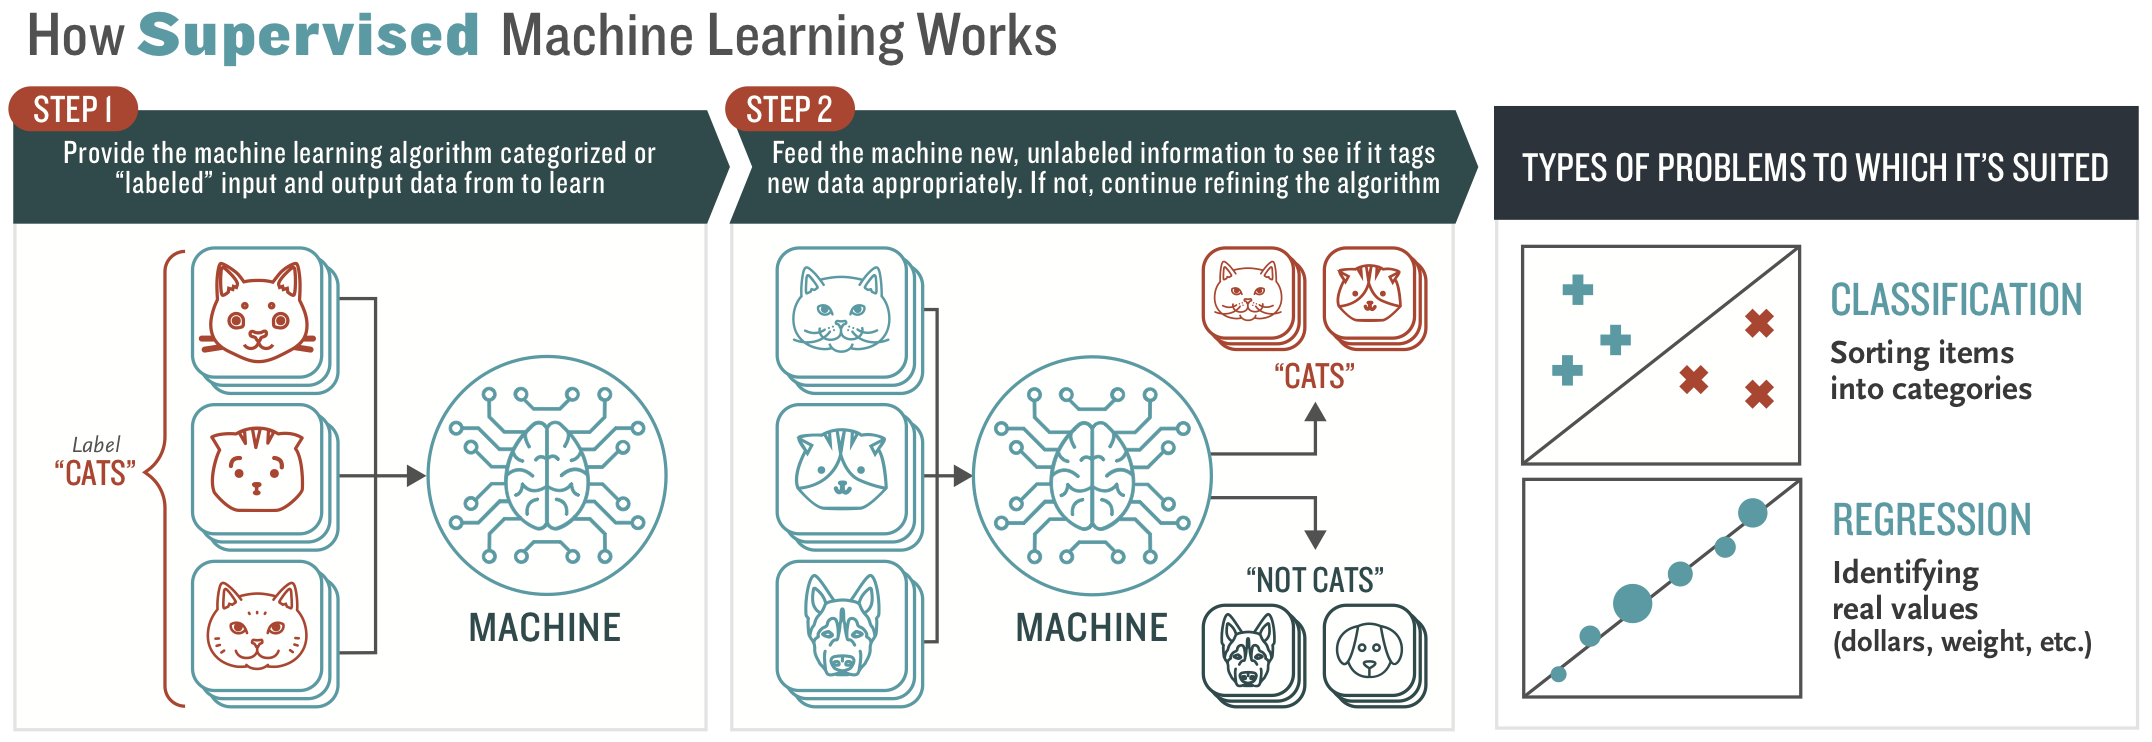
\includegraphics[width=\textwidth]{02-img-how-do-machines-learn_supervised}
      \begin{center}
        \tiny[\url{https://www.boozallen.com/content/dam/boozallen_site/sig/pdf/infographic/how-do-machines-learn.pdf}]
      \end{center}
  \end{frame}

  \begin{frame}{Info graphic unsupervised}
      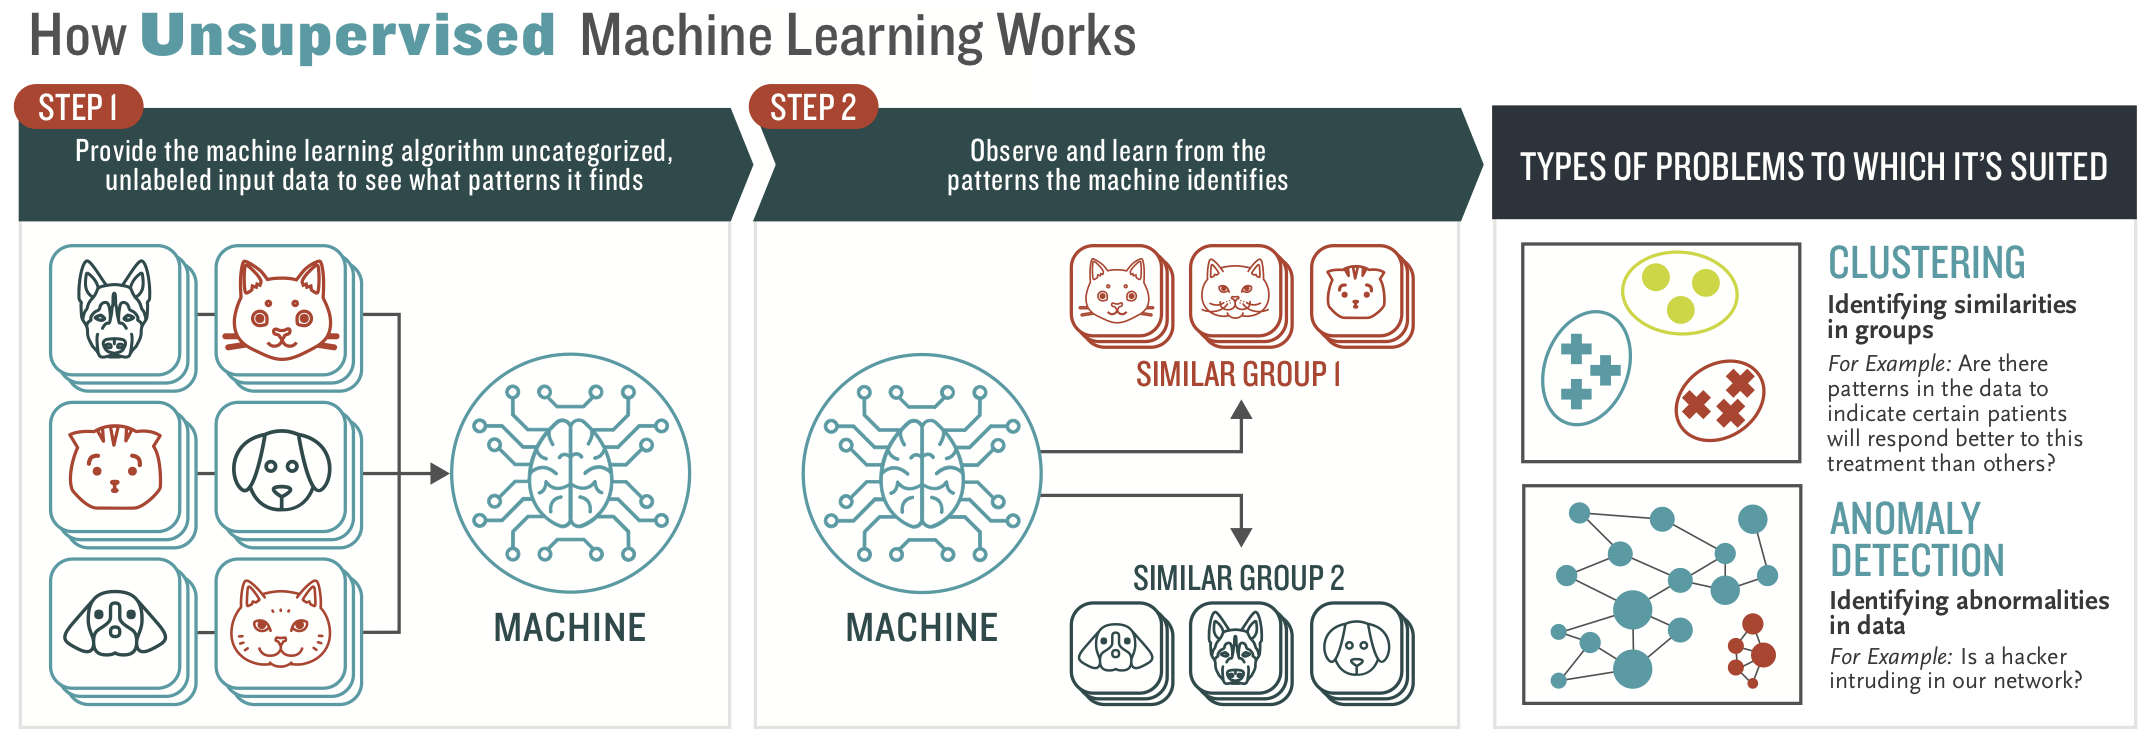
\includegraphics[width=\textwidth]{02-img-how-do-machines-learn_unsupervised}
      \begin{center}
        \tiny[\url{https://www.boozallen.com/content/dam/boozallen_site/sig/pdf/infographic/how-do-machines-learn.pdf}]
      \end{center}
  \end{frame}

  \begin{frame}{Reinforcement learning}
    \begin{columns}
      \begin{column}{0.5\textwidth}
        \begin{itemize}
          \item There is a third class of machine learning type, called \emph{reinforcement learning}
          \begin{itemize}
            \item Actually the borders are not always very clear and techniques and algorithms can end up blending concepts from multiple areas, and areas like \emph{semi-supervised learning} emerge
          \end{itemize}
          \item In reinforcement learning, the algorithm (\enquote{agent}) is presented with a reward of its actions in a given \enquote{environment} (simulation, real world task, etc.)
          \item The learner tries to tune the agent parameters so it gets a higher and higher reward when acting in the environment
          \item This field is often researched in the video game or simulation realm because new experiments can be done fast
          \begin{itemize}
            \item \url{https://deepmind.com/blog}
          \end{itemize}
        \end{itemize}
      \end{column}
      \begin{column}{0.5\textwidth}
        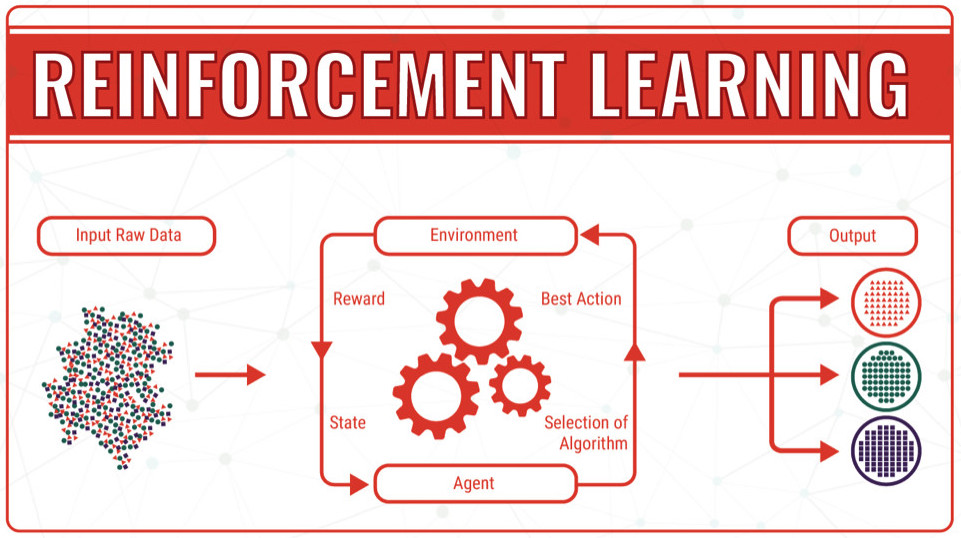
\includegraphics[width=\textwidth]{02-img-reinforcement}
        \begin{center}
          \tiny[\url{https://www.linkedin.com/pulse/machine-learning-explained-understanding-supervised-ronald-van-loon}]
        \end{center}
      \end{column}
    \end{columns}
  \end{frame}


% %%%%%%%%%%%%%%%%%%%%%%%%%%%%%%%%%%%%%%%%%%%%%%%%%%%%%%%%%%%%%%%%%%%%%%%%%%%%%
% Basics
% %%%%%%%%%%%%%%%%%%%%%%%%%%%%%%%%%%%%%%%%%%%%%%%%%%%%%%%%%%%%%%%%%%%%%%%%%%%%%
  \section{Basics}

    \begin{frame}{Performance measures}
      \begin{columns}
        \begin{column}{0.65\textwidth}
          \begin{itemize}
            \item In machine learning algorithms, the definition of the loss function is the key task to define the behaviour and the capabilities of the learned system
            \item Defining the loss can get quite complicated to find the desired result
            \item For classification tasks, usually a simple \emph{accuracy} measure is used, which is just the proportion of correctly classified samples and usually encoded using the \emph{cross-entropy loss}
            \item For regression tasks, the mean squared error is often used to measure the deviation of the model output to the data point for each sample.
              Many variants exists, for example for regularization (Huber loss)
            \item For example in a style transfer generative model, the loss is a combination from a \emph{style loss} and \emph{content loss} to produce the desired output.
          \end{itemize}
        \end{column}
        \begin{column}{0.35\textwidth}
          \vspace*{1em}
          \includegraphics[width=\textwidth]{02-img-loss_functions}
        \end{column}
      \end{columns}
    \end{frame}

    \begin{frame}{Other classifier performance metrics}
      \enlargethispage{1cm}
      \begin{columns}
        \begin{column}{0.65\textwidth}
          \begin{itemize}
            % \item For classifiers, there are other performance measures besides the value of the loss as in the regression case
            \item We can define \enquote{true positives / negatives} (TP / NP) and \enquote{false positives and negatives} (FP / NP) and show them in a truth table (\emph{confusion matrix})
            \item From these we can define some performance metrics, like
            \begin{itemize}
              \item Sensitivity: $\text{TP} / (\text{TP} + \text{FN})$
              \item Precision: $\text{TP} / (\text{TP} + \text{FP})$
              \item Fall-out: $\text{FP} / (\text{FP} + \text{TN})$
              \item Accuracy: $(\text{TP} + \text{TN}) / N_\text{data}$
              \item Note: When classes are imbalanced, these are pretty misleading (eg. $99\%$ of examples are class 0, then it's trivial to achieve $99\%$ accuracy)
            \end{itemize}
            \item Often, the area under \emph{ROC curves} is also used
            \begin{itemize}
              \item After classification, move decision boundary from $0$ to $1$ and plot fall-out against sensitivity
              \item This gives a curve from $(0,0)$ to $(1, 1)$
              \item We want that curve to have a high sensitivity even for low fall-outs, so the area should be close to one (curve should bend towards top left corner)
              \item A guessing classifier is represented by the diagonal line
            \end{itemize}
          \end{itemize}
        \end{column}
        \begin{column}{0.35\textwidth}
          \centering
          \begin{tabular}{cccc}
            & & \multicolumn{2}{c}{\small True} \\
            & & 0 & 1 \\
           \multirow{2}{*}{\STAB{\rotatebox[origin=c]{90}{
            \small Predicted
            }}}
            & 0 & \cellcolor{nordAuroraGreen} TP & \cellcolor{nordAuroraRed} FP \\
            & 1 & \cellcolor{nordAuroraRed} FN & \cellcolor{nordAuroraGreen} TN \\
          \end{tabular}

          \vspace{1cm}
          \includegraphics[width=\textwidth]{02-img-roc_curve}
        \end{column}
      \end{columns}
    \end{frame}

    \begin{frame}{Loss functions - Regression}
      \enlargethispage{1cm}
      There are few frequently used loss functions for standard regression and classification task
      \begin{description}
        \item[Mean squared error (MSE)] is the standard regression loss function
          \begin{equation*}
            \frac{1}{N} \sum_{i=1}^N \left(y_i - \hat{y}_i\right)^2
            \minter{or weighted}
            \frac{1}{N} \sum_{i=1}^N w_i\left(y_i - \hat{y}_i\right)^2
            \minter{where usually}
            w_i = \frac{1}{\sigma_i^2}
          \end{equation*}
          \begin{itemize}
            \item Penalizes large deviation from the true values quadratically
            \item Has troubles with outlier points as they tend to draw all the attention to themselves
          \end{itemize}
        \item[Mean absolute error (MAE)] is the standard regression loss function
          \begin{equation*}
            \frac{1}{N} \sum_{i=1}^N \left|y_i - \hat{y}_i\right|
          \end{equation*}
          \begin{itemize}
            \item Large deviations from the true values are only penalized linearly, more robust to outliers
            \item The \emph{Huber loss} combines MSE and MAE by switching continuously at some $\delta$
          \end{itemize}
      \end{description}
      Note: This list is not complete, see \url{https://keras.io/api/losses/} for a nice overview
    \end{frame}

    \begin{frame}{Regression loss functions example}
        \includegraphics[width=\textwidth]{02-img-regression_losses}
    \end{frame}

    \begin{frame}{Loss functions - Classification}
      \enlargethispage{1cm}
      There are few frequently used loss functions for standard regression and classification task
      \begin{description}
        \item[Binary Cross Entropy (BCE)] is the standard classification loss function for two classes
          \begin{equation*}
            - \frac{1}{N} \sum_{i=1}^N \left(
              y_i \log(\hat{y}_i) + (1 - y_i) \log(1 - \hat{y}_i) \right)
          \end{equation*}
          \begin{itemize}
            \item $y_i$ are the true, \emph{one-hot-encoded} labels, so for a point belonging to the first class, $y_i = 1$, so only the first log term survives
            \item Has troubles with outlier points as they tend to draw all the attention to themselves
          \end{itemize}
        \item[Categorial Cross Entropy] is the same thing as the BCE above, but for more than two classes.
        It generalises for $C$ classes as
          \begin{equation*}
            - \frac{1}{N}\sum_{i=1}^N \sum_{j=1}^C y_{ij} \log(\hat{y}_{ij})
          \end{equation*}
          \begin{itemize}
            \item For two classes we retrieve the BCE estimator
            \item This is also used one-hot-encoded, eg. for $4$ classes, the truth vector for a class $3$ example would be $\vec{y}_i = [0, 0, 1, 0]$
          \end{itemize}
      \end{description}
      Note: This list is not complete, see \url{https://keras.io/api/losses/} for a nice overview or \url{https://gombru.github.io/2018/05/23/cross_entropy_loss/} for a more in-depth explanation
    \end{frame}

    \begin{frame}{Overfitting / underfitting}
      \begin{itemize}
        \item A key challenge in machine learning applications is that the focus lies more on a broad validity of the model rather than trying to get the maximum information from the training set
        \item This means the trained model should also behave well on previously unseen data, not used in training
        % \item Compare: In statistic we're usually more interested in constraining some set of true parameters with the available data and model as good as possible
        \item To be able to check the performance on unseen data, a piece of the whole available data is split of and not used for training but later for checking the trained model
        \item We then have two factors that determine how well our model performs
      \end{itemize}
      \begin{description}
        \item[Underfitting] is usually meant when the model does not yield a low enough loss on training data
        \begin{itemize}
          \item This usually happens, when the model is not complex or flexible enough to capture the shape of the data distribution
          \item We say the model has a high \emph{bias} (bias regarding the   inflexibility of the model)
        \end{itemize}
        \item[Overfitting] means we have a really good performance on training data, but on unseen data, the performance is much worse
          \begin{itemize}
            \item We get overfitting, when we use a too complex model which adapts perfectly to training data, but then misses all the training data points
          \item We say the model has a high \emph{variance} (performance highly fluctuates on unseen data)
          \end{itemize}
      \end{description}
    \end{frame}

    \begin{frame}{Over- and underfitting example}
      \includegraphics[width=\textwidth]{02-img-over_underfit}
      \enlargethispage{3em}
      % \vspace{-1em}
      \emph{\footnotesize Note: For regression, line fit, polygon of 2nd and 11th order; for classification, logistic regression, plain neural net, over-fitter plain neural net without regularization and too large layers}
    \end{frame}

    \begin{frame}{Regularization}
      \begin{itemize}
        \item Consider solving a system of linear equations, if there are more variables than equation, then there is no solution to the problem
        \begin{itemize}
          \item But if we introduce artificial constraints on the parameters, we can find a solution
          \item The cost for introducing the constraints is an additional bias in the model
        \end{itemize}
        \item For a general loss function, the regularization term is simply added to the loss
          \begin{equation*}
            \frac{1}{N}\sum_{i=1}^N \mathrm{loss}_i \rightarrow
            \frac{1}{N}\sum_{i=1}^N \mathrm{loss}_i(\theta)
              + \lambda \sum_j\mathrm{reg}(\theta_j)
          \end{equation*}
          wehre $\theta$ is the regularization strength as a tunable parameter (if $0$, then we won't have regularization)
        \item Popular losses are
        \begin{itemize}
          \item L2 (\emph{ridge} or \emph{TTikhonov}) regularization: $\mathrm{reg} = \sum_j \theta_j^2$; yields parameters that are as small as possible
          \item L1 (\emph{lasso}) regularization: $\mathrm{reg} = \sum_j\left|\theta_j\right|$; yields a sparse parameter set
        \end{itemize}
        \item There are also other \enquote{effective} regularization techniques:  %, that try to minimize variance by averaging over randomized ensembles of models
        \begin{description}
          \item[Dropout] is often used in neural networks; in each training step, certain parts of the network are \enquote{turned off} simulating an average of multiple models
          \item[Bagging] is similar to dropout and often used for tree based learners; instead of turning of certain parameters, many models are trained with only a randomly sampled fraction of the data and then averaged
        \end{description}
      \end{itemize}
    \end{frame}

    \begin{frame}{Validation}
      \begin{itemize}
        \item Validation in general
        \item Cross validation
      \end{itemize}
    \end{frame}

    \begin{frame}{Hyperparamter search / tuning}
      \begin{itemize}
        \item Grid search
        \item Random search
      \end{itemize}
    \end{frame}

    \begin{frame}{Feature extraction / generation}
      \begin{itemize}
        \item PCA -> Also shortly mention as a unsupervised learner
        \item Generative algorithms
      \end{itemize}
    \end{frame}

    \begin{frame}{Feature selection}
      \begin{itemize}
        \item MRMR
        \item Forward / backward selection
      \end{itemize}
    \end{frame}

  % \subsection{Regression}

  % \begin{frame}{Intro}
  %   \begin{itemize}
  %     \item What is regression
  %     \item Loss function
  %     \item Example
  %   \end{itemize}
  % \end{frame}

  % \subsection{Classification}

  % \begin{frame}{Intro}
  %   \begin{itemize}
  %     \item What is classification
  %     \item Loss function
  %     \item Example
  %   \end{itemize}
  % \end{frame}

% %%%%%%%%%%%%%%%%%%%%%%%%%%%%%%%%%%%%%%%%%%%%%%%%%%%%%%%%%%%%%%%%%%%%%%%%%%%%%
% Example ALgoithms
% %%%%%%%%%%%%%%%%%%%%%%%%%%%%%%%%%%%%%%%%%%%%%%%%%%%%%%%%%%%%%%%%%%%%%%%%%%%%%
\section{Algorithms}
  \begin{frame}{Intro}
    \begin{itemize}
      \item On the following slides, each slide introduces a learning algorithm to get a good overview of available techniques
      \item Below are some links to get further information for the algorithms presented here and many more
      \begin{itemize}
        \item \url{https://scikit-learn.org/stable/user_guide.html}
        \item \url{http://spark.apache.org/docs/latest/ml-guide.html}
        \item \url{https://machinelearningmastery.com/a-tour-of-machine-learning-algorithms/}
        \item \url{https://towardsdatascience.com/top-10-machine-learning-algorithms-for-data-science-cdb0400a25f9}
        \item \url{https://en.wikipedia.org/wiki/Supervised_learning}
        \item \url{https://en.wikipedia.org/wiki/Unsupervised_learning}
        \item \url{https://en.wikipedia.org/wiki/Reinforcement_learning}
      \end{itemize}
    \end{itemize}
  \end{frame}

  \subsection{Supervised}

  \begin{frame}{Curve Fitting - Least Squares}
  Regression
  \end{frame}

  \begin{frame}{KNN Classification}
  Classification
  \end{frame}

  \begin{frame}{LDA Classification}
  Classification
  \end{frame}

  \begin{frame}{Support Vector Machine}
  Classification
  Regression
  \end{frame}

  \begin{frame}{Naive Bayes Classifier}
  Classification
  \end{frame}

  \begin{frame}{Tree Based Learners}
  Classification
  Regression
  \end{frame}

  \begin{frame}{Neural Networks}
  Classification
  Regression
  Only briefly
  \end{frame}

  \subsection{Unsupervised}

  \begin{frame}{Clustering}
  k-Means
  Mention DBSCAN
  \end{frame}

  \begin{frame}{Generative Neural Network Models}
  Mention GANs, Autoencoders
  \end{frame}



\end{document}
